\documentclass[margin=2cm]{standalone}

\usepackage[dvipsnames]{xcolor}
\usepackage{tikz}
\usetikzlibrary{positioning, calc}

\begin{document}
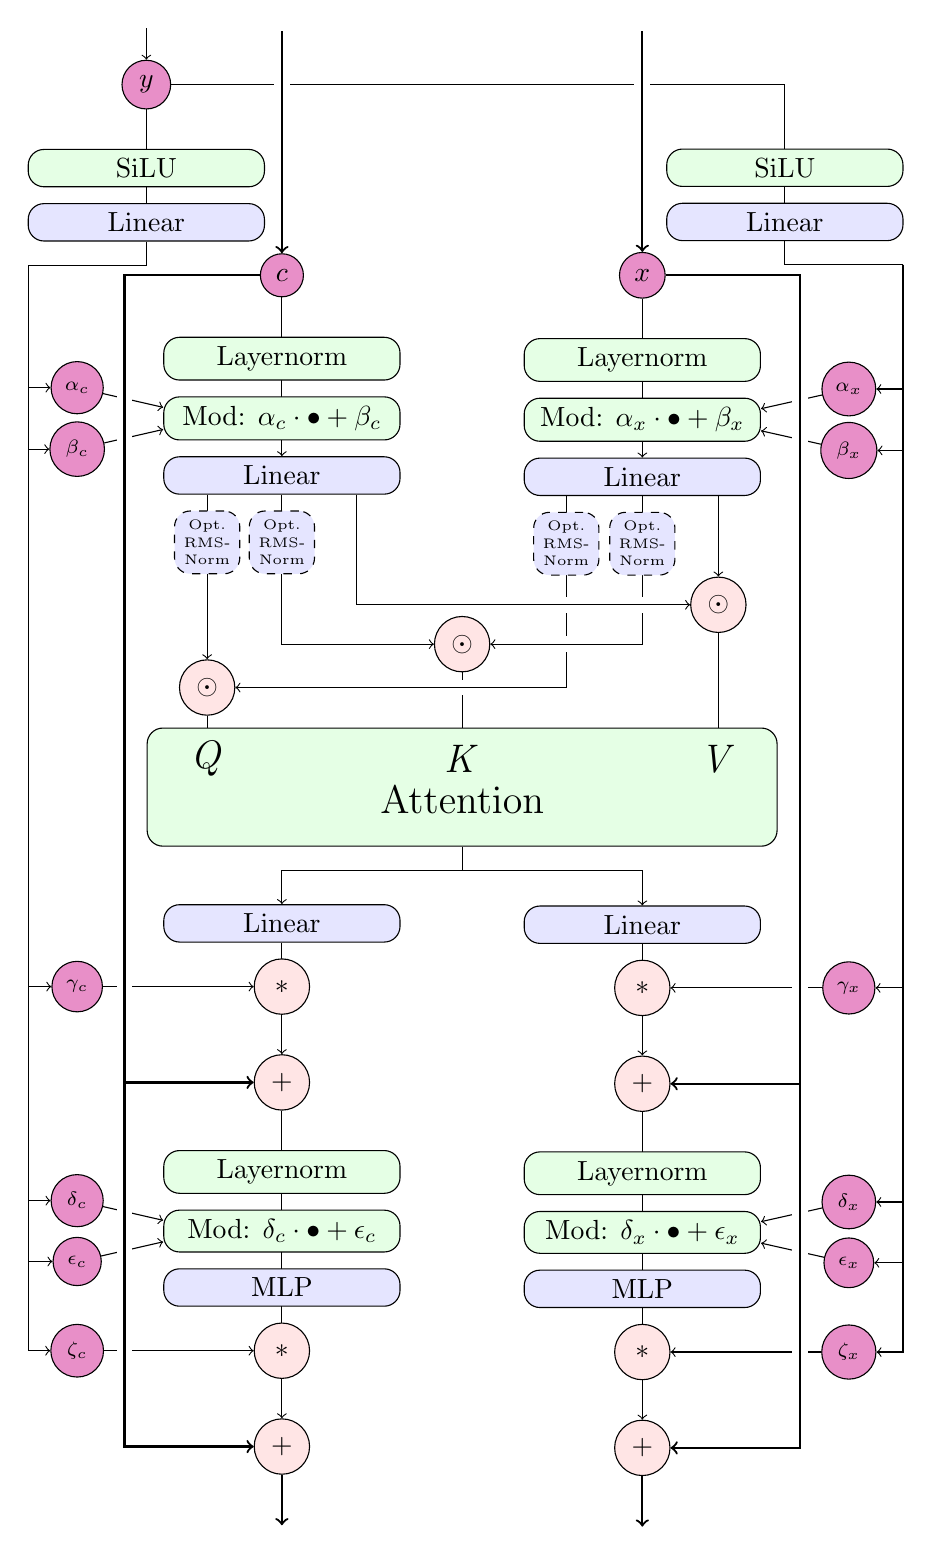
\begin{tikzpicture}[
        block/.style={draw, fill=white, rectangle, minimum width=3cm, rounded corners=0.2cm},
        trainableblock/.style={block,fill=blue!10},
        fnblock/.style={block,fill=green!10},
        operation/.style={draw, fill=red!10, circle, minimum width=2em},
        tensor/.style={draw, fill=VioletRed!50, circle},
    ]

    \pgfdeclarelayer{arrowlayer}
    \pgfdeclarelayer{residuallayer}
    \pgfsetlayers{arrowlayer,residuallayer,main}

    \newcommand{\inblockdistance}{0.2cm}
    \newcommand{\outblockdistance}{0.5cm}
    \newcommand{\attnskip}{5.2cm}
    \newcommand{\leftmodpos}{-2.6}
    \newcommand{\rightmodpos}{7.2}

    % conditional stream

    \node [tensor] (c) {$c$};
    % needed early
    \node [tensor, right=4cm of c] (x) {$x$};

    \node [below=\outblockdistance of c, fnblock] (c_ln1) {Layernorm};
    \node [below=\inblockdistance of c_ln1, fnblock] (c_mod) {Mod: $\alpha_c \cdot \bullet + \beta_c$};
    \node [below=\inblockdistance of c_mod, trainableblock] (c_lin) {Linear};

    \path let \p1=($(x)!0.5!(c)$) in node [fnblock, minimum width=8cm, minimum height=1.5cm, align=center] at (\x1, -6.5) (attn) {\vphantom{Attention}\\ \Large Attention};
    \coordinate [below=0.3cm of attn] (attn_split);
    % \node [below=\inblockdistance of attn, operation] (attn_split) {:};

    \node [below=\attnskip of c_lin, trainableblock] (c_proj) {Linear};
    \node [below=\inblockdistance of c_proj, operation] (c_proj_gated) {$*$};
    \node [below=\outblockdistance of c_proj_gated, operation] (c_attn_out) {$+$};
    \node [below=\outblockdistance of c_attn_out, fnblock] (c_ln2) {Layernorm};
    \node [below=\inblockdistance of c_ln2, fnblock] (c_mod2) {Mod: $\delta_c \cdot \bullet + \epsilon_c$};
    \node [below=\inblockdistance of c_mod2, trainableblock] (c_mlp) {MLP};
    \node [below=\inblockdistance of c_mlp, operation] (c_mlp_gated) {$*$};
    \node [below=\outblockdistance of c_mlp_gated, operation] (c_out) {$+$};

    \path let \p1=($(c_mod.north west)!0.5!(c_mod.west)+(0, 0.25)$) in node [tensor] at (\leftmodpos, \y1) (alpha_c) {$\scriptstyle \alpha_c$};
    \path let \p1=($(c_mod.south west)!0.5!(c_mod.west)-(0, 0.25)$) in node [tensor] at (\leftmodpos, \y1) (beta_c) {$\scriptstyle \beta_c$};
    \path let \p1=(c_proj_gated.west) in node [tensor] at (\leftmodpos, \y1) (gamma_c) {$\scriptstyle \gamma_c$};
    \path let \p1=($(c_mod2.north west)!0.5!(c_mod2.west)+(0, 0.25)$) in node [tensor] at (\leftmodpos, \y1) (delta_c) {$\scriptstyle \delta_c$};
    \path let \p1=($(c_mod2.south west)!0.5!(c_mod2.west)-(0, 0.25)$) in node [tensor] at (\leftmodpos, \y1) (epsilon_c) {$\scriptstyle \epsilon_c$};
    \path let \p1=(c_mlp_gated.west) in node [tensor] at (\leftmodpos, \y1) (zeta_c) {$\scriptstyle \zeta_c$};

    \node [tensor, above left=2cm and 1.3cm of c] (y) {$y$};
    \node [fnblock, below=\outblockdistance of y] (y_silu) {$\mathrm{SiLU}$};
    \node [trainableblock, below=\inblockdistance of y_silu] (y_linear) {Linear};
    \coordinate (y_split) at ($(y_linear.south)+(-1.5, -0.3)$);
    % \node [operation, below=\outblockdistance of y_linear] (y_split) {$:$};

    \coordinate (c_attn_out_left) at ($(c_attn_out) + (-2, 0)$);

    \begin{pgfonlayer}{arrowlayer}
        \draw [->] (c) -- (c_lin);
        \draw [->] (attn) -- (attn_split) -| (c_proj);
        \draw [->] (c_proj) -- (c_attn_out);
        \draw [->] (c_attn_out) -- (c_out);

        % modulation
        \draw [<-] (y.north) --++ (0, 0.4);
        \draw (y) -- (y_linear) |- (y_split);
        \draw [->] (y_split) |- (alpha_c);
        \draw [->] (y_split) |- (beta_c);
        \draw [->] (y_split) |- (gamma_c);
        \draw [->] (y_split) |- (delta_c);
        \draw [->] (y_split) |- (epsilon_c);
        \draw [->] (y_split) |- (zeta_c);

        \draw [->] (alpha_c) -- ($(c_mod.north west)!0.5!(c_mod.west)$);
        \draw [->] (beta_c) -- ($(c_mod.south west)!0.5!(c_mod.west)$);
        \draw [->] (gamma_c) -- (c_proj_gated.west);
        \draw [->] (delta_c) -- ($(c_mod2.north west)!0.5!(c_mod2.west)$);
        \draw [->] (epsilon_c) -- ($(c_mod2.south west)!0.5!(c_mod2.west)$);
        \draw [->] (zeta_c) -- (c_mlp_gated.west);

    \end{pgfonlayer}
    \begin{pgfonlayer}{residuallayer}
        % residual connections
        \draw [<-, line width=2mm, draw=white] (c) --++ (0, 3);
        \draw [->, line width=2mm, draw=white] (c) -| (c_attn_out_left) -- (c_attn_out);
        \draw [->, line width=2mm, draw=white] (c_attn_out_left) |- (c_out);
        \draw [->, line width=2mm, draw=white] (c_out) --++ (0, -1);
        \draw [<-, thick] (c) --++ (0, 3.1);
        \draw [->, thick] (c) -| (c_attn_out_left) -- (c_attn_out);
        \draw [->, thick] (c_attn_out_left) |- (c_out);
        \draw [->, thick] (c_out) --++ (0, -1);
    \end{pgfonlayer}



    % image stream

    \node [below=\outblockdistance of x, fnblock] (x_ln1) {Layernorm};
    \node [below=\inblockdistance of x_ln1, fnblock] (x_mod) {Mod: $\alpha_x \cdot \bullet + \beta_x$};
    \node [below=\inblockdistance of x_mod, trainableblock] (x_lin) {Linear};

    \node [below=\attnskip of x_lin, trainableblock] (x_proj) {Linear};
    \node [below=\inblockdistance of x_proj, operation] (x_proj_gated) {$*$};
    \node [below=\outblockdistance of x_proj_gated, operation] (x_attn_out) {$+$};
    \node [below=\outblockdistance of x_attn_out, fnblock] (x_ln2) {Layernorm};
    \node [below=\inblockdistance of x_ln2, fnblock] (x_mod2) {Mod: $\delta_x \cdot \bullet + \epsilon_x$};
    \node [below=\inblockdistance of x_mod2, trainableblock] (x_mlp) {MLP};
    \node [below=\inblockdistance of x_mlp, operation] (x_mlp_gated) {$*$};
    \node [below=\outblockdistance of x_mlp_gated, operation] (x_out) {$+$};

    \path let \p1=($(x_mod.north east)!0.5!(x_mod.east)+(0, 0.25)$) in node [tensor] at (\rightmodpos , \y1) (alpha_x) {$\scriptstyle \alpha_x$};
    \path let \p1=($(x_mod.south east)!0.5!(x_mod.east)-(0, 0.25)$) in node [tensor] at (\rightmodpos , \y1) (beta_x) {$\scriptstyle \beta_x$};
    \path let \p1=(x_proj_gated.east) in node [tensor] at ( \rightmodpos , \y1) (gamma_x) {$\scriptstyle \gamma_x$};
    \path let \p1=($(x_mod2.north east)!0.5!(x_mod2.east)+(0, 0.25)$) in node [tensor] at (\rightmodpos , \y1) (delta_x) {$\scriptstyle \delta_x$};
    \path let \p1=($(x_mod2.south east)!0.5!(x_mod2.east)-(0, 0.25)$) in node [tensor] at (\rightmodpos , \y1) (epsilon_x) {$\scriptstyle \epsilon_x$};
    \path let \p1=(x_mlp_gated.east) in node [tensor] at (\rightmodpos , \y1) (zeta_x) {$\scriptstyle \zeta_x$};

    \coordinate [above right=2cm and 1.6cm of x] (yx) {};
    % \node [tensor, above right=2cm and 1.3cm of x] (y) {$y$};
    \node [fnblock, below=0.6cm of yx] (y_silu) {$\mathrm{SiLU}$};
    \node [trainableblock, below=\inblockdistance of y_silu] (y_linear) {Linear};
    \coordinate (y_split) at ($(y_linear.south)+(1.5, -0.3)$);
    % \node [operation, below=\outblockdistance of y_linear] (y_split) {$:$};

    \coordinate (x_attn_out_left) at ($(x_attn_out) + (2, 0)$);

    \begin{pgfonlayer}{arrowlayer}
        \draw [->] (x) -- (x_lin);
        \draw [->] (attn) -- (attn_split) -| (x_proj);
        \draw [->] (x_proj) -- (x_attn_out);
        \draw [->] (x_attn_out) -- (x_out);

        % modulation
        \draw (y) -| (yx) -- (y_linear) |- (y_split);
        \draw [->] (y_split) |- (alpha_x);
        \draw [->] (y_split) |- (beta_x);
        \draw [->] (y_split) |- (gamma_x);
        \draw [->] (y_split) |- (delta_x);
        \draw [->] (y_split) |- (epsilon_x);
        \draw [->] (y_split) |- (zeta_x);

        \draw [->] (alpha_x) -- ($(x_mod.north east)!0.5!(x_mod.east)$);
        \draw [->] (beta_x) -- ($(x_mod.south east)!0.5!(x_mod.east)$);
        \draw [->] (gamma_x) -- (x_proj_gated.east);
        \draw [->] (delta_x) -- ($(x_mod2.north east)!0.5!(x_mod2.east)$);
        \draw [->] (epsilon_x) -- ($(x_mod2.south east)!0.5!(x_mod2.east)$);
        \draw [->] (zeta_x) -- (x_mlp_gated.east);

    \end{pgfonlayer}
    \begin{pgfonlayer}{residuallayer}
        % residual connections
        \draw [<-, line width=2mm, draw=white] (x) --++ (0, 3);
        \draw [->, line width=2mm, draw=white] (x) -| (x_attn_out_left) -- (x_attn_out);
        \draw [->, line width=2mm, draw=white] (x_attn_out_left) |- (x_out);
        \draw [->, line width=2mm, draw=white] (x_out) --++ (0, -1);
        \draw [<-, thick] (x) --++ (0, 3.1);
        \draw [->, thick] (x) -| (x_attn_out_left) -- (x_attn_out);
        \draw [->, thick] (x_attn_out_left) |- (x_out);
        \draw [->, thick] (x_out) --++ (0, -1);
    \end{pgfonlayer}


    \node [below=0.1cm of attn.north] (k) {\Large \emph{K}};
    \node [left= 2.9cm of k.center] (q) {\Large \emph{Q}};
    \node [right=2.9cm of k.center] (v) {\Large \emph{V}};
    \node [above=0.2cm of q, operation] (q_join) {$\odot$};
    \node [above=0.8cm of k, operation] (k_join) {$\odot$};
    \node [above=1.3cm of v, operation] (v_join) {$\odot$};

    \coordinate (x_lin_vout) at (x_lin.south -| v_join);
    \coordinate (x_lin_kout) at (x_lin.south);
    \coordinate (x_lin_qout) at ($(x_lin_kout)+(x_lin_kout)-(x_lin_vout)$);

    \coordinate (c_lin_qout) at (c_lin.south -| q_join);
    \coordinate (c_lin_kout) at (c_lin.south);
    \coordinate (c_lin_vout) at ($(c_lin_kout)+(c_lin_kout)-(c_lin_qout)$);

    % \node [above=0.7cm of q.center, fnblock, dashed, align=center, minimum width=0cm] (q_norm) {Optional \\ RMS-Norm};
    % \node [above=0.7cm of k.center, fnblock, dashed, align=center, minimum width=0cm] (k_norm) {Optional \\ RMS-Norm};
    \node [below=\inblockdistance of c_lin_qout, trainableblock, dashed, minimum width=0cm, align=center] (q_norm_c) {\tiny Opt.\\[-0.2cm]\tiny RMS-\\[-0.2cm] \tiny Norm};
    \node [below=\inblockdistance of c_lin_kout, trainableblock, dashed, minimum width=0cm, align=center] (k_norm_c) {\tiny Opt.\\[-0.2cm]\tiny RMS-\\[-0.2cm] \tiny Norm};
    \node [below=\inblockdistance of x_lin_qout, trainableblock, dashed, minimum width=0cm, align=center] (q_norm_x) {\tiny Opt.\\[-0.2cm]\tiny RMS-\\[-0.2cm] \tiny Norm};
    \node [below=\inblockdistance of x_lin_kout, trainableblock, dashed, minimum width=0cm, align=center] (k_norm_x) {\tiny Opt.\\[-0.2cm]\tiny RMS-\\[-0.2cm] \tiny Norm};


    \begin{pgfonlayer}{arrowlayer}
        \draw (k_join) -- (k);

        \draw [->] (c_lin_qout) -| (q_join);
        \draw [line width=2mm, white] (x_lin_qout) |- (q_join);
        \draw [->] (x_lin_qout) |- (q_join);
        \draw (q_join) -- (q);

        \draw [->] (c_lin_kout) |- (k_join);
        \draw [line width=2mm, white] (x_lin_kout) |- (k_join);
        \draw [->] (x_lin_kout) |- (k_join);
        % k_join -- k is above

        \draw [line width=2mm, white] (c_lin_vout) |- (v_join);
        \draw [->] (c_lin_vout) |- (v_join);
        \draw [->] ($(x_lin)+(0.25, 0)$) -| (v_join);
        \draw [->] (v_join) -- (v);
    \end{pgfonlayer}
\end{tikzpicture}
\end{document}
